\setcounter{ex}{0}
\section{Giá trị lớn nhất và nhỏ nhất của hàm số}
\subsection{Đề 1}
\Opensolutionfile{ans}[ans/ans-2-B2]
\caulc
\begin{ex}%[Câu 1]%[2D1N3-2]
	Cho hàm số liên tục trên $\mathbb{R}$ thỏa mãn giá trị nhỏ nhất của hàm số trên $\mathbb{R}$ là $2$. Khẳng định nào sau đây là đúng?
	\choice
	{$f(x)<2$, $\forall x\in \mathbb{R}$}
	{$f(x)>2$, $\forall x\in \mathbb{R}$}
	{\True $f(x)\ge 2$, $\forall x\in \mathbb{R}$, $\exists x_0\colon f(x_0)=2$}
	{$f(x)\le 2$, $\forall x\in \mathbb{R}$, $\exists x_0\colon f(x_0)=2$}
	\loigiai{
		Theo định nghĩa giá trị nhỏ nhất của hàm số, chọn đáp án $$f(x)\ge 2,\,\forall x\in \mathbb{R},\,\exists x_0\colon f(x_0)=2.$$}
\end{ex}
\begin{ex}%[Câu 2]%[2D1N3-2]
	Hàm số nào dưới đây có giá trị lớn nhất trên $\mathbb{R}$?
	\choice
	{$y=x^4-2x^2$}
	{$y=-3x^3+x^2-5$}
	{$y=x^3+3x^2-7x+1$}
	{\True $y=-2x^4-x^2+5$}
	\loigiai{
		\begin{itemize}
			\item $\lim\limits_{x\to +\infty}(x^4-2x^2)=+\infty$ suy ra hàm số $y=x^4-2x^2$ không có giá trị lớn nhất trên $\mathbb{R}$. (Loại)
			\item $\lim\limits_{x\to -\infty}(-3x^3+x^2-5)=+\infty$ suy ra hàm số $y=-3x^3+x^2-5$ không có giá trị lớn nhất trên $\mathbb{R}$. (Loại)
			\item $\lim\limits_{x\to +\infty}(x^3+3x^2-7x+1)=+\infty$ suy ra hàm số $y=x^3+3x^2-7x+1$ không có giá trị lớn nhất trên $\mathbb{R}$. (Loại)
			\item $y=-2\left(x^2+\dfrac{1}{4}\right)^2+\dfrac{21}{4}\le \dfrac{41}{8}$. Do đó hàm số $y$ có giá trị lớn nhất bằng $\dfrac{41}{8}$ khi $x=0$.
		\end{itemize}
		}
\end{ex}
\begin{ex}%[Câu 3]%[2D1H3-1]
	Tìm giá trị lớn nhất $M$ của hàm số $y=\dfrac{3x-1}{x-3}$ trên đoạn $[0;2]$.
	\choice
	{\True $M=\dfrac{1}{3}$}
	{$M=-\dfrac{1}{3}$}
	{$M=5$}
	{$M=-5$}
	\loigiai{
		Trên đoạn $[0;2]$, ta có $y'=-\dfrac{8}{(x-3)^2}<0$, $\forall x\in (0;2)$ và $y'=0$ vô nghiệm. \\
		Vì $y(0)=\dfrac{1}{3}$; $y(2)=-5$ nên $M=\max\limits_{[0;2]} y=\dfrac{1}{3}$.}
\end{ex}
\begin{ex}%[Câu 4]%[2D1H3-2]
	Giá trị lớn nhất của hàm số $y=-x^3+3x+1$ trên khoảng $(0;+\infty)$ bằng
	\choice
	{$1$}
	{\True $3$}
	{$-1$}
	{$5$}
	\loigiai{
		Ta có $y'=-3x^2+3$, $y'=0\Leftrightarrow \hoac{&x=1\in (0;+\infty) \\&x=-1\notin (0;+\infty).}$\\
		Bảng biến thiên
		\begin{center}
			
\begin{tikzpicture}[line cap=round, line join=round,font=\footnotesize,>=stealth, scale=1]
			\tkzTabInit[nocadre=false,lgt=1.2,espcl=2.5,deltacl=0.6]
			{$x$ /0.6,$y’$ /0.6,$y$ /1.5}
			{$0$,$1$, $+\infty$}
			\tkzTabLine{,+,0,-,}
			\tkzTabVar{-/$1$,+/$3$,-/$-\infty$ }
		\end{tikzpicture}
		\end{center}
		Từ bảng biến thiên ta thấy $\max\limits_{[0;+\infty)}f(x)=3$.}
\end{ex}
\begin{ex}%[Câu 5]%[2D1H3-1]
	Gọi $M$, $m$ lần lượt là giá trị lớn nhất, giá trị nhỏ nhất của\\
	 hàm số $f(x)=x^4-2x^2+3$ trên đoạn $[0;2]$. Tổng $M+m$ bằng
	\choice
	{$11$}
	{$14$}
	{$5$}
	{\True $13$}
	\loigiai{
		Tập xác định $\mathscr{D}=\mathbb{R}$ và $f'(x)=4x^3-4x$.\\
		Ta có $f'(x)=0\Leftrightarrow 4x^3-4x=0\Leftrightarrow \hoac{&x=0\in [0;2] \\&x=-1\notin [0;2] \\&x=1\in [0;2].}$\\
		Lại có $f(0)=3;f(1)=2;f(2)=11$. Do đó $\heva{&M=11 \\&m=2}\Rightarrow M+m=13$.}
\end{ex}
\begin{ex}%[Câu 6]%[2D1H3-1]
	Trên đoạn $[0;3]$, hàm số $y=-x^3+3x$ đạt giá trị lớn nhất tại điểm
	\choice
	{$x=0$}
	{$x=3$}
	{\True $x=1$}
	{$x=2$}
	\loigiai{
		Tập xác định $\mathscr{D}=\mathbb{R}$.\\
		Ta có $y'=-3x^2+3$ và $y'=0\Leftrightarrow -3x^2+3=0\Leftrightarrow \hoac{&x=1\in (0;3) \\&x=-1\notin (0;3).}$\\
		Ta có $y(0)=0;y(1)=2;y(3)=-18$.\\
		Vậy $\max\limits_{[0;3]}y=y(1)=2$.}
\end{ex}
\begin{ex}%[Câu 7]%[2D1N3-2]
	Cho hàm số $y=f(x)$ có bảng biến thiên trên khoảng $(1;+\infty)$ như sau.
	\begin{center}
		
\begin{tikzpicture}[line cap=round, line join=round,font=\footnotesize,>=stealth, scale=1]
			\tkzTabInit[lgt=1.2,espcl=3]
			{$x$/1.2,$f’(x)$/1.2,$f(x)$/2.5}
			{$-\infty$,$1$,$2$,$+\infty$}
			\tkzTabLine{,h,,-,z,+,}
			\tkzTabVar{-H/,+/$+\infty$,-/$5$,+/$+\infty$}
	\end{tikzpicture}
	\end{center}
	Giá trị nhỏ nhất của hàm $y=f(x)$ trên khoảng $(1;+\infty)$ là
	\choice
	{không tồn tại}
	{$1$}
	{$2$}
	{\True $5$}
	\loigiai{
		Dựa vào bảng biến thiên ta thấy hàm số có giá trị nhỏ nhất $\min\limits_{(1;+\infty)}f(x)=5$ khi $x=2$.}
\end{ex}
\begin{ex}%[Câu 8]%[2D1N3-2]
	Cho hàm số $y=f(x)$ xác định và liên tục trên $[-1;1]$ và có bảng biến thiên như sau
	\begin{center}
		
\begin{tikzpicture}[line cap=round, line join=round,font=\footnotesize,>=stealth, scale=1]
			\tkzTabInit[nocadre=false,lgt=1.2,espcl=2.5,deltacl=0.6]
			{$x$ /0.6,$y’$ /0.6,$y$ /1.5}
			{$-1$,$0$, $1$}
			\tkzTabLine{,+,0,-,}
			\tkzTabVar{-/$0$,+/$1$,-/$\dfrac{2}{3}$ }
		\end{tikzpicture}
	\end{center}
	Giá trị lớn nhất của hàm $y=f(x)$ trên đoạn $[-1;1]$ là
	\choice
	{\True $1$}
	{$\dfrac{2}{3}$}
	{không tồn tại}
	{$0$}
	\loigiai{
		Dựa vào bảng biến thiên ta thấy $\max\limits_{[-1;1]}f(x)=1$ khi $x=0$.}
\end{ex}
\begin{ex}%[Câu 9]%[2D1N3-2]
	Cho hàm số $y=f(x)$ có bảng biến thiên trên $[-5;7)$ như sau
	\begin{center}
		
\begin{tikzpicture}[line cap=round, line join=round,font=\footnotesize,>=stealth, scale=1]
			\tkzTabInit[nocadre=false,lgt=1.2,espcl=2.5,deltacl=0.6]
			{$x$ /0.6,$y’$ /0.6,$y$ /1.5}
			{$-5$,$1$, $7$}
			\tkzTabLine{,-,0,+,d,}
			\tkzTabVar{+/$6$,-/$2$,+D/$9$ }
		\end{tikzpicture}
	\end{center}
	Mệnh đề nào dưới đây đúng?
	\choice
	{$\min\limits_{[-5;7)}f(x)=6$}
	{\True $\min\limits_{[-5;7)}f(x)=2$}
	{$\max\limits_{[-5;7)}f(x)=9$}
	{$\max\limits_{[-5;7)}f(x)=6$}
	\loigiai{
		Dựa vào bảng biến thiên trên $[-5;7)$, ta có $\min\limits_{[-5;7)}f(x)=f(1)=2$.}
\end{ex}
\begin{ex}%[Câu 10]%[2D1H3-2]
	\immini[thm]
	{Cho hàm số $y=f(x)$ xác định và liên tục trên $\mathbb{R}$ có đồ thị như hình vẽ bên. Tìm giá trị nhỏ nhất $m$ và giá trị lớn nhất $M$ của hàm số $y=f(x)$ trên đoạn $[-2;2]$.
		\choice[2]
		{\True $m=-5$; $M=-1$}
		{$m=-2$; $M=2$}
		{$m=-1$; $M=0$}
		{$m=-5$; $M=0$}}
	{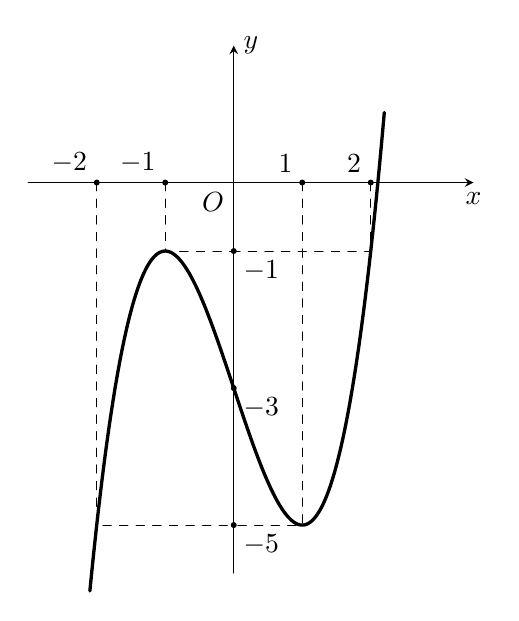
\begin{tikzpicture}[>=stealth,scale=.87, line join = round, line cap = round]
			\draw[->] (-3,0) -- (0,0) node[below left]{$O$}--(3.5,0) node[below]{$x$};
			\draw[->] (0,-5.7) --(0,2) node[right]{$y$};
			\foreach \x in {-2,-1,1,2} {
				\filldraw (\x,0) circle (1pt) node[above left]{$\x$};
			}
			\foreach \y in {-5,-3,-1} {
				\filldraw (0,\y) circle (1pt) node[below right]{$\y$};
			}
			\draw[dashed] (-2,0)--(-2,-5)--(0,-5)  (-1,0)--(-1,-1)--(0,-1)  (1,0)--(1,-5)--(0,-5)  (2,0)--(2,-1)--(0,-1);
			\draw [thick,line width=1.2,domain=-2.1:2.2,samples=300]plot(\x,{1*(\x)^(3)-3*(\x)-3});
	\end{tikzpicture}}
	\loigiai{
		Từ đồ thị ta thấy $\heva{&M=\max\limits_{[-2;2]}f(x)=-1 \\&m=\min\limits_{[-2;2]}f(x)=-5}$.}
\end{ex}
\begin{ex}%[Câu 11]%[2D1H3-1]
	\immini[thm]
	{Cho hàm số $f(x)$ liên tục trên $[-1;5]$ và có đồ thị trên đoạn $[-1;5]$ như hình vẽ bên. Tổng giá trị lớn nhất và giá trị nhỏ nhất của hàm số $f(x)$ trên đoạn $[-1;5]$ bằng
	\choice[2]
	{$-1$}
	{$4$}
	{\True $1$}
	{$2$}}
	{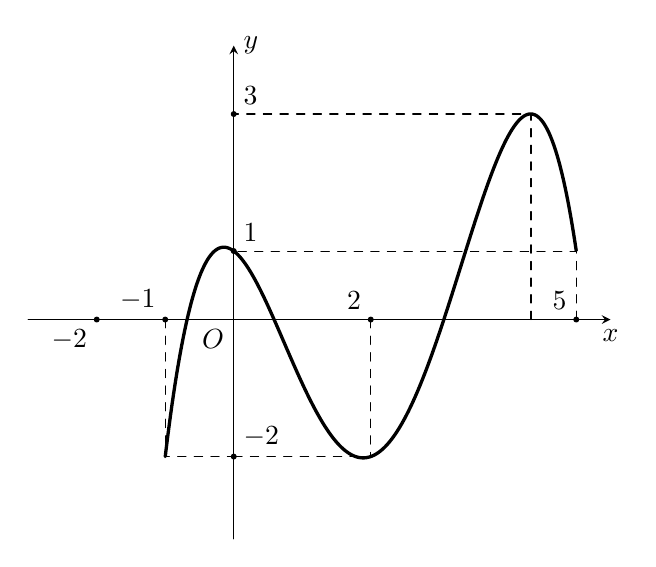
\begin{tikzpicture}[>=stealth,scale=.87, line join = round, line cap = round]
			\draw[->] (-3,0) -- (0,0) node[below left]{$O$}--(5.5,0) node[below]{$x$};
			\draw[->] (0,-3.2) --(0,4) node[right]{$y$};
			\foreach \x in {-1,2,5} {
				\filldraw (\x,0) circle (1pt) node[above left]{$\x$};
			}
			\foreach \y in {-2,1,3} {
				\filldraw (0,\y) circle (1pt) node[above right]{$\y$};
			}
			\filldraw (-2,0) circle (1pt) node[below left]{$-2$};
			\draw[dashed] (-1,0)--(-1,-2)--(0,-2)  (2,0)--(2,-2)--(0,-2)  (5,0)--(5,1)--(0,1)  (4.34,0)--(4.34,3)--(0,3);
			\draw [thick,line width=1.2,domain=-1:5,samples=300]plot(\x,{0-0.158314*(\x)^(4)+1.28322*(\x)^(3)-2.30827*(\x)^(2)-0.749805*(\x)+1});
	\end{tikzpicture}}
	\loigiai{
		Từ đồ thị ta thấy $\heva{&M=\max\limits_{[-1;5]}f(x)=3 \\&m=\min\limits_{[-1;5]}f(x)=-2}\Rightarrow M+m=1$.}
\end{ex}
\begin{ex}%[Câu 12]%[2D1H3-1]
	\immini[thm]
	{Cho hàm số $y=f(x)$ liên tục trên đoạn $[1;6]$ và có đồ thị như hình vẽ bên.
	Gọi $M$ và $m$ lần lượt là giá trị lớn nhất và nhỏ nhất của hàm số đã cho trên đoạn $[1;6]$. Giá trị của $M-m$ bằng
	\choice[2]
	{\True $5$}
	{$-8$}
	{$-9$}
	{$8$}}
	{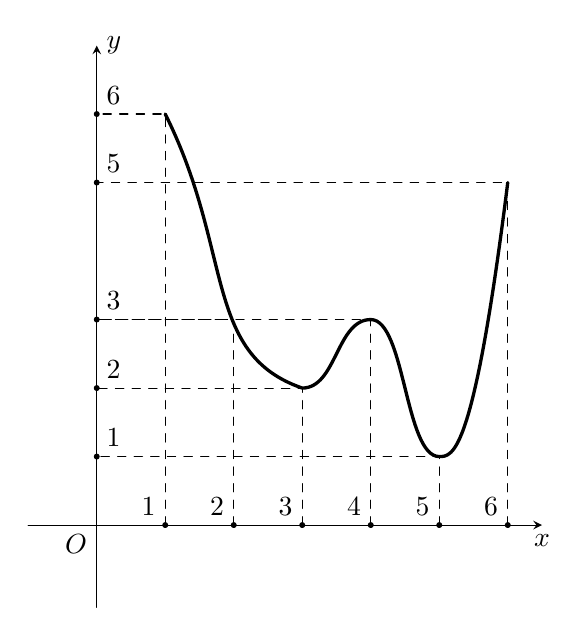
\begin{tikzpicture}[>=stealth,scale=.87, line join = round, line cap = round]
			\draw[->] (-1,0) -- (0,0) node[below left]{$O$}--(6.5,0) node[below]{$x$};
			\draw[->] (0,-1.2) --(0,7) node[right]{$y$};
			\foreach \x in {1,2,3,4,5,6} {
				\filldraw (\x,0) circle (1pt) node[above left]{$\x$};
			}
			\foreach \y in {1,2,3,5,6} {
				\filldraw (0,\y) circle (1pt) node[above right]{$\y$};
			}
			\draw[dashed] (1,0)--(1,6)--(0,6);
			\draw[dashed] (2,0)--(2,3)--(0,3);
			\draw[dashed] (3,0)--(3,2)--(0,2);
			\draw[dashed] (4,0)--(4,3)--(0,3);
			\draw[dashed] (5,0)--(5,1)--(0,1);
			\draw[dashed] (6,0)--(6,5)--(0,5);
			\draw[thick,line width=1.2] (1,6)..controls (2,4) and (1.55,2.5)..(3,2)..controls (3.5,2) and (3.5,3)..(4,3)..controls (4.5,3) and (4.5,1)..(5,1)..controls (5.2,1) and (5.5,1)..(6,5);
	\end{tikzpicture}}
	\loigiai{
		Từ đồ thị suy ra $1\le f(x)\le 6$, $\forall x\in [1;6]$.\\
		 Và $f(5)=1$; $f(1)=6 \Rightarrow \heva{&M=6 \\&m=1}\Rightarrow M-m=5$.}
\end{ex}
\Closesolutionfile{ans}
\indapan{6}{ans/ans-2-B2}
\cauds
\Opensolutionfile{ans}[ans/ans-2-B2-DS]
\begin{ex}%[Câu 13]%[2D1H3-2]
	Cho hàm số $y=f(x)$ có bảng biến thiên trên đoạn $[-2;3]$ như sau
	\begin{center}
		
\begin{tikzpicture}
			\tkzTabInit[nocadre=false,lgt=1.2,espcl=2.5,deltacl=0.6]
			{$x$ /.6,$g'(x)$ /.6,$g(x)$ /2}{$-2$,$-1$,$1$,$3$}
			\tkzTabLine{,+,$0$,-,$0$,+,}
			\tkzTabVar{-/$0$ ,+/$1$,-/$-3$,+/$7$}
		\end{tikzpicture}
	\end{center}
	\choiceTF
	{\True Hàm số đạt giá trị nhỏ nhất bằng $-3$ trên đoạn $[-2;3]$}
	{\True Hàm số đạt giá trị lớn nhất tại điểm $x=-1$ trên khoảng $(-2;1)$}
	{Hàm số đạt giá trị nhỏ nhất tại $x=-3$}
	{Trên khoảng $(-2;3)$ ta có $\max\limits_{(-2;3)}y=7$}
	\loigiai{
	Dựa vào bảng biến thiên, ta có
	\begin{itemchoice}
		\itemch \textbf{Đúng}. Hàm số đạt giá trị nhỏ nhất bằng $-3$ trên đoạn $ [ -2;3]$. 
		\itemch\textbf{ Đúng}. Hàm số đạt giá trị lớn nhất tại điểm $x=-1$ trên khoảng $(-2;1)$. 
		\itemch \textbf{Sai}. Hàm số đạt giá trị nhỏ nhất tại $x=-3$. Vì $-3\notin [ -2;3]$ nên hàm số không thể đạt giá trị nhỏ nhất tại $x=-3$.
		\itemch \textbf{Sai}. Trên khoảng $(-2;3)$ ta có $\max\limits_{(-2;3)}y=7$. Quan sát bảng biến thiên, ta thấy $y=7$ tại $x=3$. Tuy nhiên $3\notin (-2;3)$, do đó không tồn tại $\max\limits_{(-2;3)}y=7$.
	\end{itemchoice}}
	\end{ex}
\begin{ex}%[Câu 14]%[2D1H3-2]
	Cho hàm số $y=\sqrt{x+1}$ có bảng biến thiên sau
	\begin{center}
\begin{tikzpicture}[line cap=round, line join=round,font=\footnotesize,>=stealth, scale=1]
			\tkzTabInit[nocadre=false,lgt=1.2,espcl=2.5,deltacl=0.6]
			{$x$ /0.7,$y’$ /0.6,$y$ /2}
			{$-1$, $+\infty$}
			\tkzTabLine{d,-,}
			\tkzTabVar{-/$0$,+/$+\infty$}
	\end{tikzpicture}\end{center}
	\choiceTF
	{Hàm số không có giá trị nhỏ nhất}
	{Hàm số có giá trị lớn nhất}
	{Hàm số có giá trị nhỏ nhất bằng $-1$}
	{\True Hàm số có giá trị nhỏ nhất bằng $0$}
	\loigiai{
	Dựa vào bảng biến thiên, ta có
	\begin{itemchoice}
		\itemch \textbf{Sai}. Hàm số có giá trị nhỏ nhất bằng $0$.
		\itemch \textbf{Sai}. Hàm số có giá trị lớn nhất.
		\itemch \textbf{Sai}. Hàm số có giá trị nhỏ nhất bằng $-1$.
		\itemch \textbf{Đúng}. Hàm số có giá trị nhỏ nhất bằng $0$. Hàm số đạt giá trị nhỏ nhất tại $x=-1$.
	\end{itemchoice}
}
\end{ex}
\begin{ex}%[Câu 15]%[2D1H3-2]
	Cho hàm số $y=f(x)$ có đồ thị như sau
	\begin{center}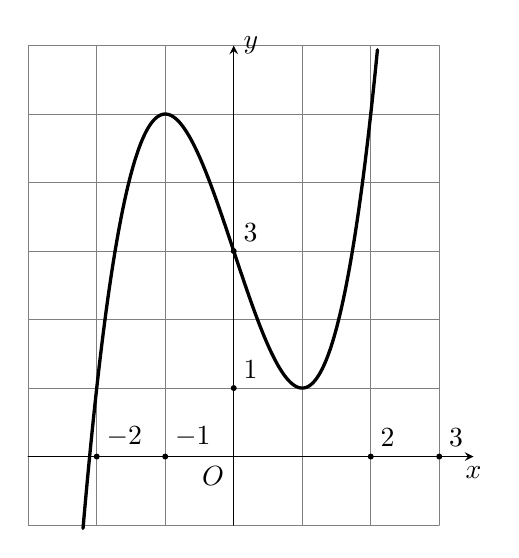
\begin{tikzpicture}[>=stealth,scale=.87, line join = round, line cap = round]
			\draw[step=1.0,black,very thin,gray] (-3,-1) grid (3,6);
			\draw[->] (-3,0) -- (0,0) node[below left]{$O$}--(3.5,0) node[below]{$x$};
			\draw[->] (0,-1) --(0,6) node[right]{$y$};
			\foreach \x in {-2,-1,2,3} {
				\filldraw (\x,0) circle (1pt) node[above right]{$\x$};
			}
			\foreach \y in {1,3} {
				\filldraw (0,\y) circle (1pt) node[above right]{$\y$};
			}
			\draw [thick,line width=1.2,domain=-2.2:2.1,samples=300]plot(\x,{1*(\x)^(3)-3*(\x)+3});
		\end{tikzpicture}
	\end{center}
	\choiceTF
	{\True Hàm số không có giá trị lớn nhất và giá trị nhỏ nhất}
	{Hàm số đạt giá trị lớn nhất bằng $5$}
	{\True Hàm số có $\min \limits_{[0;2]}y=1$}
	{\True Hàm số có $\min \limits_{[-2;2]}y=1$ và $\max \limits_{[-2;2]}y=5$}
\loigiai{
	Dựa vào đồ thị, ta thấy
	\begin{itemchoice}
		\itemch \textbf{Đúng}. Vì $\lim\limits_{x\to +\infty}y=+\infty$ và $\lim\limits_{x\to -\infty}y=-\infty$.
		\itemch \textbf{Sai}. Vì $\lim\limits_{x\to +\infty}y=+\infty$.
		\itemch \textbf{Đúng}. Hàm số có $\min \limits_{[0;2]}y=1$.
		\itemch \textbf{Đúng}. Hàm số có $\min \limits_{[-2;2]}y=1$ và $\max \limits_{[-2;2]}y=5$.
	\end{itemchoice}
}
\end{ex}
\begin{ex}%[Câu 16]%[2D1H3-2]
	Cho hàm số $y=x-\sqrt{x-1}$ có bảng biến thiên sau
\begin{center}
\begin{tikzpicture}[line cap=round, line join=round,font=\footnotesize,>=stealth, scale=1]
		\tkzTabInit[nocadre=false,lgt=1.2,espcl=2.5,deltacl=0.6]
		{$x$ /0.87,$y’$ /0.6,$y$ /2}
		{$1$, $\dfrac{5}{4}$, $+\infty$}
		\tkzTabLine{,-,z,+,}
		\tkzTabVar{+/$1$,-/$\dfrac{3}{4}$,+/$0$}
\end{tikzpicture}\end{center}
	\choiceTF
	{Hàm số có giá trị nhỏ nhất bằng $\dfrac{3}{4}$ và không có giá trị lớn nhất}
	{\True Hàm số có giá trị nhỏ nhất bằng $\dfrac{3}{4}$ và giá trị lớn nhất bằng $1$}
	{Hàm số không có giá trị lớn nhất và giá trị nhỏ nhất}
	{Hàm số đạt giá trị nhỏ nhất tại điểm có hoành độ $x=1$ và giá trị nhỏ nhất bằng $1$}
	\loigiai{
		\begin{itemchoice}
			\itemch \textbf{Sai}. Vì hàm số có giá trị nhỏ nhất bằng $\dfrac{3}{4}$ và có giá trị lớn nhất nhất bằng $1$.
			\itemch \textbf{Đúng}. Hàm số có giá trị nhỏ nhất bằng $\dfrac{3}{4}$. Ta có $y(1)=1> \lim\limits_{x\to +\infty}y=0$. Suy ra hàm số có giá trị lớn nhất bằng $1$ tại $x=1$.
			\itemch \textbf{Sai}. Vì hàm số có giá trị nhỏ nhất bằng $\dfrac{3}{4}$ và có giá trị lớn nhất bằng $1$.
			\itemch \textbf{Sai}. Vì hàm số có giá trị nhỏ nhất bằng $\dfrac{3}{4}$ và có giá trị lớn nhất bằng $1$.
		\end{itemchoice}
	}
\end{ex}
\Closesolutionfile{ans}
\indapan{3}{ans/ans-2-B2-DS}
\Opensolutionfile{ans}[ans/ans-2-B2-KQ]
\caukq
\begin{ex}%[Câu 17]%[2D1H3-6]
Ông Nam cần xây dựng một bể chứa nước có dạng hình hôp chữ nhật không có nắp đậy để phục vụ cho viêc tưới cây trong vườn. Do các điều kiện về diện tích vườn, ông Nam cần bể có thể tích là $36$ m$^3$, đáy bể có chiều dài gấp hai lần chiều rộng và chiều rộng không quá $4$ m, biết rằng chi phí vật liệu xây dựng mỗi mét vuông diện tích bề mặt là như nhau. Hỏi chiều cao bể nước bằng bao nhiêu để tổng chi phí vật liệu là nhỏ nhất?
\shortans{$2$}
\loigiai{
	\immini[thm]
	{Xem bể chứa có dạng hình hộp chữ nhật $ABCD.A'B'C'D'$ như hình vẽ.\\
		Gọi $x$ (m) là chiều rộng của bể, ta có $0<x \leq 4$. Chiều dài của bể là $2x$ (m).\\
Gọi $h$ (m) là chiều cao bể nước, ta có thể tích của bể là $V=x \cdot (2x) \cdot h$.\\
Suy ra $h=\dfrac{V}{2 x^2}=\dfrac{36}{2 x^2}=\dfrac{18}{x^2}$ (m).}
{\begin{tikzpicture}[scale=0.6, font=\footnotesize,line join=round, line cap=round, >=stealth]
		\path 
		(0,0) coordinate (A)
		++(-130:3) coordinate (B)
		++(0:6) coordinate (C)
		($(A)+(C)-(B)$) coordinate (D)
		($(A)!1/2!(C)$) coordinate (O)
		;
		\foreach \i in {A,B,C,D}{
			\coordinate (\i') at ($(\i)+(0,4)$);
		}
		\draw (A')--(B')--(C')--(D')--cycle;
		\draw (C)--node[below right]{$x$}(D);
		\draw (C)--node[below]{$2x$}(B);
		\draw (B)--(B') (C)--(C') (D)--(D')  (B)--(C)--(D);
		\draw[dashed,thin](B)--(A)--(A') (B)--(A)--(D);
		\foreach \i/\g in {A'/90,B'/90,C'/90,D'/90,A/-90,B/-90,C/-90,D/-90}
		\fill[black] (\i) circle(1pt)+(\g:5mm)node[scale=1]{$\i$};
\end{tikzpicture}}
Tổng diện tích các mặt cần xây là
$$
\begin{aligned}
	& S=S_{A B C D}+2 \cdot S_{A B B' A'}+2 \cdot S_{B C C'B'} \\
	& =2 x^2+2 \cdot x \cdot \dfrac{18}{x^2}+2\cdot 2 x \cdot \dfrac{18}{x^2}=2 x^2+\dfrac{108}{x}.
\end{aligned}
$$
Xét hàm số $S(x)=2 x^2+\dfrac{108}{x}$ với $(0<x \leq 4)$, ta có
$$
\begin{aligned}
	& S'(x)=4 x-\dfrac{108}{x^2}=\dfrac{4 x^3-108}{x^2}=\dfrac{4(x-3)(x^2+3 x+9)}{x^2} . \\
	& S'(x)=0 \Leftrightarrow x=3.
\end{aligned}
$$
Do $x^2>0$ và $x^2+3 x+9>0$ khi $x \in (0 ; 4]$ nên dấu của $S'(x)$ trên $(0 ; 4]$ phụ thuôc dấu của biểu thức $x-3$.
Bảng biến thiên
\begin{center}
	
\begin{tikzpicture}[line cap=round, line join=round,font=\footnotesize,>=stealth, scale=1]
		\tkzTabInit[nocadre=false,lgt=1.2,espcl=2.5,deltacl=0.6]
		{$x$ /0.87,$S'(x)$ /0.6,$S(x)$ /2}
		{$0$, $3$, $4$}
		\tkzTabLine{,-,z,+,}
		\tkzTabVar{+/,-/$54$,+/}
\end{tikzpicture}
\end{center}
Chi phí vât liêu xây dưng thấp nhất khi tổng diên tích các mặt cần xây $S(x)$ là nhỏ nhất. Dưa vào bảng biến thiên, ta có $S(x)$ đạt giá tri nhỏ nhất tại $x=3$, suy ra $h=2$.\\
Vậy cần xây bể có chiều cao là $2$ (m).}
\end{ex}
\begin{ex}%[Câu 18]%[2D1H3-6]
	Ông $A$ dự định sử dụng hết $5$ m$^2$ kính để làm bể cá bằng kính có dạng hình hộp chữ nhật không nắp, chiều dài gấp đôi chiều rộng. Bể cá có thể tích lớn nhất bằng bao nhiêu?
	\shortans{$1{,}01$}
	\loigiai{
	Gọi chiều rộng của bể cá là $x$ với $x>0$.\\
	Ông $A$ dùng hết $5$ m$^2$ kính để làm bể cá nên $2x^2+6xh=5\Rightarrow h=\dfrac{5-2x^2}{6x}$.\\
	Do $x>0$ và $h>0$ nên $0<x<\sqrt{\dfrac{5}{2}}$.\\ Thể tích bể cá $V=\dfrac{1}{3}(5x-2x^3)$.\\
	Ta có $V'=\dfrac{1}{3}(5-6x^2)$, $V'=0\Rightarrow x=\sqrt{\dfrac{5}{6}}$.\\ Bảng biến thiên của $V$ là
	\begin{center}
\begin{tikzpicture}[line cap=round, line join=round,font=\footnotesize,>=stealth, scale=1]
			\tkzTabInit[nocadre=false,lgt=1.2,espcl=2.5,deltacl=0.6]
			{$x$ /0.87,$v'(x)$ /0.6,$v(x)$ /2}
			{$0$, $\sqrt{\tfrac{5}{6}}$, $\sqrt{\tfrac{5}{2}}$}
			\tkzTabLine{,+,z,-,}
			\tkzTabVar{-/$0$,+/$1{,}01$,-/$0$}
	\end{tikzpicture}\end{center}
	Từ bảng biến thiên suy ra bể cá có thể tích lớn nhất bằng $1,01$ m$^3$.}
\end{ex}
\begin{ex}%[Câu 19]%[2D1H3-6]
	Một chất điểm chuyển động theo phương trình $S=-t^3+9t^2+t+10$ trong đó $t$ tính bằng $(s)$ và $S$ tính bằng $(m)$. Thời gian để vận tốc của chất điểm đạt giá trị lớn nhất là bao nhiêu?
	\shortans{$3$}
\loigiai{
	Ta có $v=S'=-3t^2+18t+1=-3(t-3)^2+28\le 28$, $\forall t>0$.\\
	Dấu \lq\lq $=$\rq\rq\,  xảy ra khi $t=3$.\\
	Vậy vận tốc của chất điểm đạt giá trị lớn nhất bằng $28$ khi $t=3$.}
\end{ex}
\begin{ex}%[Câu 20]%[2D1H3-6]
	Một vật chuyển động theo quy luật $s=-2t^3+24t^2+9t-3$ với $t$ là khoảng thời gian tính từ lúc bắt đầu chuyển động và $s$ là quãng đường vật đi được trong khoảng thời gian đó. Hỏi trong khoảng thời gian $10$ giây, kể từ lúc bắt đầu chuyển động, vận tốc lớn nhất của vật đạt được bằng bao nhiêu?
\shortans{$105$}
	\loigiai{
	Ta có $v=s'=-6t^2+48t+9$.\\
	Theo đề, ta cần tìm vận tốc lớn nhất trong 10 giây đầu tiên nên bài toán trở thành tìm giá trị lớn nhất của hàm số $v(t)=-6t^2+48t+9$ trên đoạn $[0;10]$.\\
	Khi đó $v'(t)=-12t+48$, $v'(t)=0\Leftrightarrow t=4\in [0;10]$.\\
	Ta có $v(0)=9$; $v(4)=105$; $v(10)=-111$. Suy ra $v_{\max}=105$ (m/s).\\
	Vậy vận tốc lớn nhất của vật đạt được trong khoảng $10$ giây đầu tiên là $105$ (m/s).}
\end{ex}
\begin{ex}%[Câu 21]%[2D1H3-6]
	Một chất điểm chuyển động theo quy luật $s=-t^3+6t^2+17t$, với $t$ là khoảng thời gian tính từ lúc vật bắt đầu chuyển động và $s$ là quãng đường vật đi được trong khoảng thời gian đó. Khi đó vận tốc $v$ (m/s) của chuyển động đạt giá trị lớn nhất trong khoảng $8$ giây đầu tiên bằng bao nhiêu?
	\shortans{$29$}
\loigiai{
	Ta có $v(t)=s'(t)=-3t^2+12t+17$.\\
	Ta có $v'(t)=-6t+12=0\Leftrightarrow t=2$.\\
	Xét trong khoảng $8$ giây đầu tiên, nghĩa là $t\in [0;8]$, bảng biến thiên của hàm số $v(t)$ là
	\begin{center}
\begin{tikzpicture}[line cap=round, line join=round,font=\footnotesize,>=stealth, scale=1]
			\tkzTabInit[nocadre=false,lgt=1.2,espcl=2.5,deltacl=0.6]
			{$t$ /0.87,$v'(t)$ /0.6,$v(t)$ /2}
			{$0$, $2$, $8$}
			\tkzTabLine{,+,z,-,}
			\tkzTabVar{-/$17$,+/$29$,-/$-79$}
	\end{tikzpicture}\end{center}
	Vậy $\max \limits_{[0;8]}v(t)=29$ (m/s) tại thời điểm $t=2$.}
\end{ex}
\begin{ex}%[Câu 22]%[2D1H3-6]
	Một chất điểm chuyển động theo phương trình $S=-t^3+3t^2-2$, trong đó $t$ tính bằng giây và $S$ tính theo mét. Chuyển động có vận tốc lớn nhất là bao nhiêu?
\shortans{$3$}
	\loigiai{
	$S=-t^3+3t^2-2\Rightarrow v=-3t^2+6t=-3(t-1)^2+3\le 3$.\\
	Do đó $\max v=3$ (m/s).}
\end{ex}

\Closesolutionfile{ans}
\indapan{6}{ans/ans-2-B2-KQ}